\subsection*{What removes relay}

Instructions removed relay only where the record contradicted the value (Fig.~\ref{fig:mechanism}a--c). On the chemistry cell in which three fields agreed with a wrong weight but the formula contradicted it, dropping the registered instruction to use the provided tools lowered relay from 80--91\% to 34--51\% for three of four models ($p \le 4\times10^{-9}$), and a sentence stating that the database contains errors and that the formula is authoritative lowered it to 0--1\% for all four. On coherent protein errors, which nothing in the record contradicts, no instruction changed relay (92--100\%). An output format that asked for the database value and the agent's own estimate separately did reach coherent errors for two models (relay 98\% to 52\% for Opus~5, 96\% to 0\% for Argon; DeepSeek 94\% to 90\%), presumably by licensing the memory that the probe shows these models hold, but it gave no reliable audit trail: the stated database value matched the record in only 0--28\% of runs on the protein cell. Memory decided the matter once a conflict was visible: with a second source shown, proteins whose remembered length was the superseded one were relayed far more often than those whose remembered length was today's (Opus~5, 13 of 21 against 2 of 144; DeepSeek, 17 of 18 against 38 of 150; $p \le 10^{-8}$; Fig.~\ref{fig:mechanism}e).

A harness can act on the record before the agent sees it (Methods). Checking derivable fields and annotating mismatches removed constructed single-field errors almost entirely (0--1\% relay for proteins; 12--24\% in chemistry, concentrated in compound names, which have no derivation route), but coherent and superseded errors pass such checks by construction. For those we compared each record with a second copy: AlphaFold DB \cite{varadi2024alphafolddb,jumper2021alphafold}, which takes its sequences from current UniProt and so tests a stale record against a current one rather than providing independent evidence, and NCI CACTUS for compounds, which agreed with PubChem's formula for 270 of the 283 compounds it resolved. Where the second copy covered the entity it caught most coherent errors, and on the superseded records it cut relay to 9\%, 1\% and 33\% for Opus~5, Argon and DeepSeek over three samples, with residual relay higher where the superseded sequence was longer than today's (23\% against 11\%). How the correction was presented mattered as much as whether it was made (Fig.~\ref{fig:present}). Writing the corrected value into the record while listing the original in a note left 3--11\% relay; labelling the original explicitly as the original database value made Argon choose it in 41\% of runs; correcting the record silently left nothing to relay (0 of 702 runs), with accuracy at 99\% (234 of 237 runs per model, the misses all on the one protein the second copy did not cover). Without any second source, a harness that withheld every derivable field failing its check, with no note, left 0 of 709 corrupted numeric fields relayed, with accuracy of 93--100\% on proteins (DeepSeek 79--84\% if its unparsed runs are counted as wrong) and 83--95\% in chemistry, where the remaining errors were compound names, which are not withheld (Fig.~\ref{fig:mechanism}f).

\begin{figure}[p]
\centering
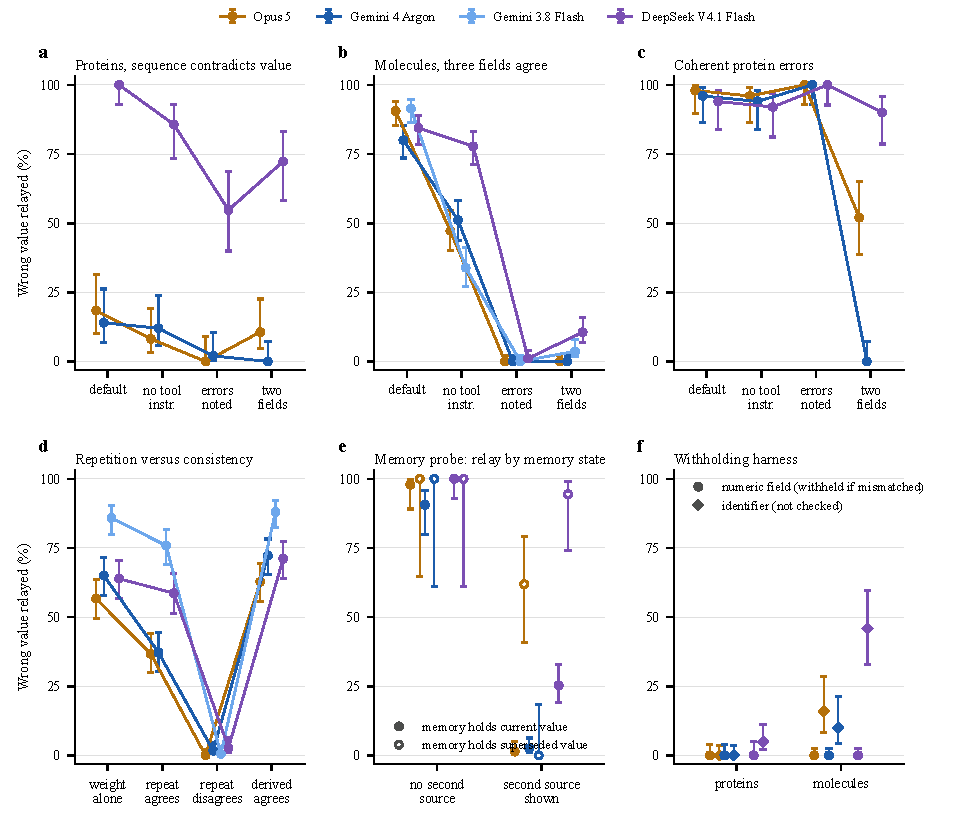
\includegraphics[width=\linewidth]{../figures/nmi_mechanism.pdf}
\caption{\textbf{What turns detection into override.} \textbf{a--c}, Relay under four system prompts: the registered default; without the instruction to use the tools (no tool instr.); with a note that the database contains errors and the sequence or formula is authoritative (errors noted); with the answer and the record's value asked for as separate fields (two fields) on three cells: protein tasks whose full record contradicts the value (\textbf{a}), the chemistry agreement cell with three fields agreeing with the wrong weight, three samples (\textbf{b}), and coherent protein errors that nothing in the record contradicts (\textbf{c}). \textbf{d}, Agreement versus repetition: relay of a wrong molecular weight alone, with a derived field (heavy-atom count) that agrees, and with a verbatim copy that agrees or disagrees under an unfamiliar (molecular weight reported) or familiar (average mass) field name; 60 compounds, three samples, familiar-name arms one sample. \textbf{e}, Memory probe: relay of the superseded value for proteins whose memory held the current (filled) or the superseded (open) length, without a second source (full record) and with the second source shown (three samples). \textbf{f}, Withholding harness: relay of corrupted numeric fields, withheld when they fail the derivation check (circles), and of identifiers, which the harness does not check (diamonds); impossible and plausible pooled. Markers give relay with 95\% Wilson intervals; lines connect one model.}

\label{fig:mechanism}
\end{figure}
\begin{figure}[t]
\centering
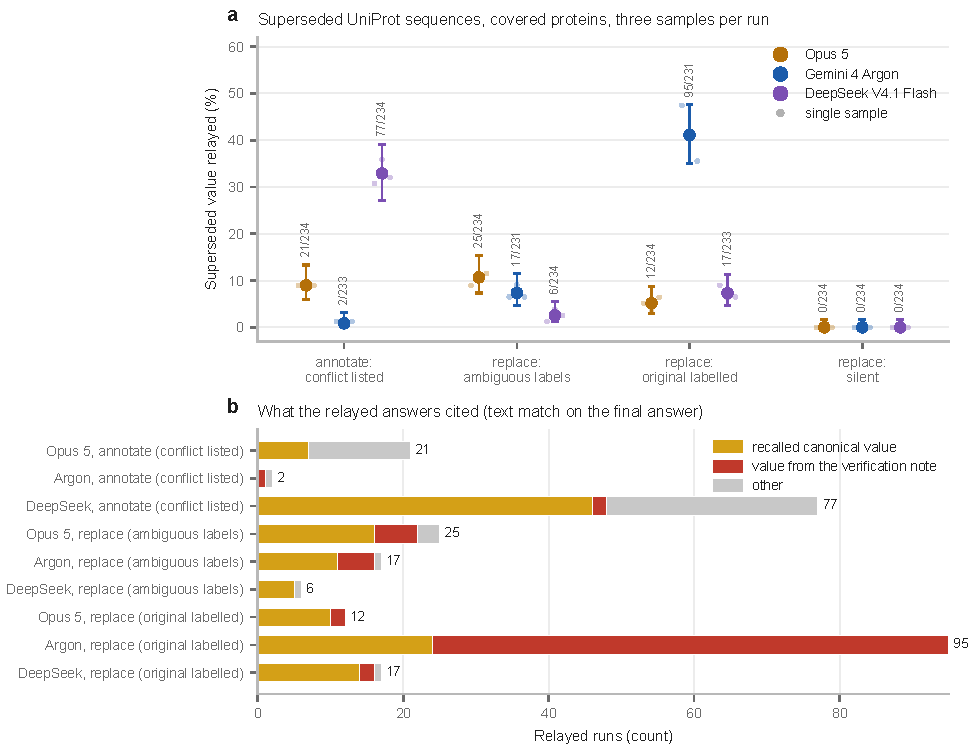
\includegraphics[width=\linewidth]{../figures/nmi_presentation.pdf}
\caption{\textbf{Correcting the record works; showing the conflict does not.} \textbf{a}, Relay of superseded values on covered proteins under four presentations of the second source (three samples per run; 95\% Wilson intervals; small dots, single samples; counts above). \textbf{b}, What the relayed answers cited, by a text match on the final answer: a recalled canonical value, the original or observed value shown in the verification note, or neither.}

\label{fig:present}
\end{figure}
